\documentclass[a4paper]{article} 

%中文环境设置
\usepackage{xeCJK} 
\usepackage{indentfirst}
\setlength{\parindent}{2em}
\usepackage{enumitem}

\usepackage{abstract}
\renewcommand{\abstractname}{摘要}
\providecommand{\keywords}[1]{\textbf{\textit{关键词}} #1}

\setCJKmainfont{STSong} % 中文主字体设置 

\usepackage[colorlinks,linkcolor=blue, citecolor=blue]{hyperref}

% 常用宏包
\usepackage{float}
\usepackage{stfloats}
\usepackage{graphicx}
\usepackage{color}
\usepackage{supertabular}

% 代码环境设置
\usepackage{listings}
\lstset{
	columns=fullflexible,
 	frame=single,
 	breaklines=true,
}
\definecolor{lightgray}{gray}{0.9}
\newcommand{\inlinecode}[2]{\colorbox{lightgray}{\lstinline[language=#1]$#2$}}

% 页面段落设置
\usepackage{multicol}
\usepackage{geometry}
\geometry{left=3.18cm, right=3.18cm, top=2.54cm, bottom=2.54cm}
\linespread{1.3}
%\setlength{\parskip}{0.5em} 

% 数学环境设置
\usepackage{amsmath}
\usepackage{amsthm}
\usepackage{amsfonts}
\newtheorem{myDef}{Definition} 
\newtheorem{myThm}{Theorem}
\newtheorem{myProp}{Property}

\begin{document} 
\title{非线性方程组求根实验题}
\author{吴佳龙 2018013418}
\date{}
\maketitle

\begin{abstract}
	结合理论分析和编程计算,运用不同算法求解非线性方程,并比较他们的优劣。运用的算法分别为不动点迭代法、Steffensen 迭代法和 Newton 迭代法。
\end{abstract}

%\keywords{one, two, three, four}

\begin{multicols}{2}

\begin{section}{问题}

	求解非线性方程组 \begin{equation}
		x^{3}+2 x^{2}+10 x-20=0
		\label{equ}
	\end{equation} 在 $x_0=1$ 附近的根。准确解为$x^{*}=1.368808107 \cdots$,希望精度达到 $10^{-7}$
	
\end{section}

\begin{section}{不动点迭代法}

	\begin{subsection}{算法原理}
		
		将方程 $f(x)=0$ 改写为 $x=\varphi(x)$ 。设定初始值 $x_0$,迭代 $$x_{k+1} = \varphi(x_k), k=1,2,\cdots$$
		
	\end{subsection}

	\begin{subsection}{收敛性分析}
		
		设 $x^*$ 为函数 $\varphi$ 的不动点,$\varphi^\prime$ 在 $x^*$ 的某个邻域 $S$ 上存在且连续,且 $|\varphi^\prime (x^*)|<1$,则不动点迭代法局部收敛。
		
		若存在常数 $L\in (0,1)$,在区域内满足 $$|\varphi(x) - \varphi(y)|\leq L|x-y|, \forall x,y\in S$$,则不动点迭代法产生的序列满足 $$|x^* - x_k| \leq {L \over 1-L} |x_{k}-x_{k-1}|$$
		
	\end{subsection}
	
	\begin{subsection}{算法实现}
		
		不动点迭代法的 MATLAB 实现如下:
		
		\begin{lstlisting}[language=Matlab]
function [x, x_series] = myFixedPoint(x0, phi, eps, kmax)
% 不动点迭代法 解 x=phi(x)
% kmax: 最大迭代次数
% eps: 相邻两次迭代结果小于eps,则终止

x = x0;
x_series = [x0];
for k = 1:kmax
    last_x = x;
    x = phi(last_x);
    x_series = [x_series x];
    if abs(x-last_x) < eps
        break
    end
end
end	
		\end{lstlisting}
		
	\end{subsection}
	
	\begin{subsection}{计算结果}
		对于方程 \ref{equ},分别选择迭代函数:\begin{equation} 
			x_{k+1}=\varphi_1(x_k) = \frac{20-2 x_{k}^{2}-x_{k}^{3}}{10}
			\label{func1}
		\end{equation} 
		\begin{equation} 
			x_{k+1}=\varphi_2(x_k) = \sqrt[3]{20-10 x_{k}-2 x_{k}^{2}}
			\label{func2}
		\end{equation}
		
		调用函数 
		\begin{lstlisting}[language=Matlab]
myFixedPoint(1, @(x)(20-2*x^2-x^3)/10.0, 1e-8, 50)
		\end{lstlisting} 和
		 
		\begin{lstlisting}[language=Matlab]
myFixedPoint(1, @(x)nthroot(20-10*x-2*x^2,3), 1e-8, 50)
		\end{lstlisting} 计算。迭代产生的序列如表 \ref{table_fp} 所示。
		
		可以看到 $\varphi_1$ 和 $\varphi_2$ 产生的迭代序列都不收敛,这是由于 $|\varphi_1^\prime(x^*)|$ 和 $|\varphi_2^\prime(x^*)|$ 的绝对值都大于 $1$,不满足局部收敛的条件。
	
		\begin{table}[H]
		\caption{不动点迭代法}
		\centering
		\label{table_fp}
		\begin{tabular}{l|l|l}
		\hline
		       & $\varphi_1$ \ref{func1} & $\varphi_2$ \ref{func2} \\ \hline
		$x_0$  & 1.0                            & 1.0                            \\
		$x_1$  & 1.7                            & 2.0                            \\
		$x_2$  & 0.9307                         & -2.0                           \\
		$x_3$  & 1.74614203626                  & 3.17480210394                  \\
		$x_4$  & 0.857796793737                 & -3.17171550601                 \\
		$x_5$  & 1.78971892824                  & 3.1614381025                   \\
		$x_6$  & 0.78611746376                  & -3.16164373894                 \\
		$x_7$  & 1.82782332719                  & 3.16233360997                  \\
		$x_8$  & 0.721147914713                 & -3.16231990025                 \\
		$x_9$  & 1.85848552855                  & 3.16227393009                  \\
		$x_{10}$ & 0.66729126817                  & -3.16227484407                 \\
		$x_{11}$ & 1.8812314848                   & 3.16227790884                  \\
		$x_{12}$ & 0.626419796624                 & -3.16227784791                 \\
		$x_{13}$ & 1.89693882451                  & 3.16227764359                  \\
		$x_{14}$ & 0.597734533785                 & -3.16227764765                 \\
		$x_{15}$ & 1.90718643312                  & 3.16227766127                  \\
		$x_{16}$ & 0.578815600138                 & -3.162277661                   \\
		$x_{17}$ & 1.91360258592                  & 3.16227766009                  \\ \hline
		\end{tabular}
		\end{table}
		
	\end{subsection}

\end{section}


\begin{section}{Steffensen 迭代法}

	\begin{subsection}{算法原理}
		
		将 Aitken 加速方法和不动点迭代法结合起来就得到了 Steffensen 迭代法。
		
		$$\left\{\begin{array}{l}{y_{k}=\varphi\left(x_{k}\right)} \\ {z_{k}=\varphi\left(y_{k}\right)} \\ {x_{k+1}=x_{k}-\frac{\left(y_{k}-x_{k}\right)^{2}}{z_{k}-2 y_{k}+x_{k}}}\end{array}\right.$$
		
		Steffensen迭代法可以看做将 $(x_k, \varepsilon(x_k)=y_k-x_k )$ 和 $(y_k, \varepsilon(y_k)=z_k-y_k )$ 连结延长到与x轴的交点作为新的近似值 $x_{k+1}$。
		
	\end{subsection}

	\begin{subsection}{收敛性分析}
		
		根据课本上的定理 2.3:
		
		\begin{myThm}
			设函数 $\varphi$ 是不动点迭代法的迭代函数,$x^*$ 是 $\varphi$ 的不动点,在 $x^*$ 邻域 $\varphi$ 有 $p+1$ 阶导数存在且连续,对 $p=1$,若 $\varphi^\prime(x^*)\neq 1$,则 Steffensen 方法是二阶的。若不动点迭代法是 $p(>1)$ 阶收敛的,则 Steffensen 方法是 $2p-1$ 阶收敛的。 
		\end{myThm}
		
		这说明,Steffensen 方法可以把不收敛的不动点迭代法改进为二阶收敛的方法。
		
	\end{subsection}
	
	\begin{subsection}{算法实现}
	
		Steffensen加速方法的 MATLAB 实现如下:
		
		\begin{lstlisting}[language=Matlab]
function [x, x_series] = mySteffensen(x0, phi, eps, kmax)
% Steffensen加速方法 解 x=phi(x)
% kmax: 最大迭代次数
% eps: 相邻两次迭代结果小于eps,则终止

x = x0;
x_series = [x0];
for k = 1:kmax
    last_x = x;
    y = phi(x);
    z = phi(y);
    x = x- (y-x)^2/(z-2*y+x);
    x_series = [x_series x];
    if abs(x-last_x) < eps
        break
    end
end
end	
		\end{lstlisting}

	\end{subsection}
	
	\begin{subsection}{计算结果}
	
		对于 $\varphi_1$ 和 $\varphi_2$ 分别调用
		\begin{lstlisting}[language=Matlab]
mySteffensen(1, @(x)(20-2*x^2-x^3)/10.0, 1e-8, 50)
		\end{lstlisting} 和
		\begin{lstlisting}[language=Matlab]
mySteffensen(1, @(x)nthroot(20-10*x-2*x^2,3), 1e-8, 50)
		\end{lstlisting} 计算。产生的迭代序列如表 \ref{table_steff} 所示。
		
		\begin{table}[H]
		\caption{Steffensen 迭代法}
		\centering
		\label{table_steff}
		\begin{tabular}{l|l|l}
		\hline
		      & $\varphi_1$ \ref{func1} + Steffensen & $\varphi_2$ \ref{func2} + Steffensen \\ \hline
		$x_0$ & 1.0                                                   & 1.0                                                   \\
		$x_1$ & 1.2                                                   & 1.33349213911                                         \\
		$x_2$ & 1.27374039955                                         & 1.36841543911                                         \\
		$x_3$ & 1.30830003901                                         & 1.36880805831                                         \\
		$x_4$ & 1.34727521974                                         & 1.36880810782                                         \\
		$x_5$ & 1.36672391381                                         & 1.36880810782                                         \\
		$x_6$ & 1.36878928488                                         &                                                       \\
		$x_7$ & 1.36880810629                                         &                                                       \\
		$x_8$ & 1.36880810782                                         &                                                      
		\end{tabular}
		\end{table}

		可以看到,Steffensen 方法将原来不收敛的不动点迭代法改进为收敛的算法,且是二阶收敛。
		
	\end{subsection}
	
\end{section}

\begin{section}{Newton 迭代法}

	\begin{subsection}{算法原理}
		
		为求解方程 $f(x)=0$,等价于求函数 $f(x)$ 的零点,Newton 法对曲线上的点 $(x_k, f(x_k))$ 作切线,切线与 x 轴的焦点作为新的近似值。
		
		$$x_{k+1} = x_k - {f(x_k)\over f^\prime(x_{k})}$$
		
	\end{subsection}

	\begin{subsection}{收敛性分析}
		
		有课本上定理 4.1 :
		
		\begin{myThm}
			设 $f(x^*)=0,f^\prime(x^*) \neq 0$,且 $f$ 在包含 $x^*$ 的一个区间上有二阶连续导数,则 Newton 迭代法局部收敛到 $x^*$,且至少二阶收敛,并有
			
			$$\lim_{k \rightarrow \infty} {x_{k+1}-x^*\over (x_k-x^*)^2} = {f^{\prime\prime}(x^*) \over 2f^\prime(x^*)}$$
		\end{myThm}

	\end{subsection}
	
	\begin{subsection}{算法实现}
	
		Newton 法的 MATLAB 实现如下:
		
		\begin{lstlisting}[language=Matlab]
function [x, x_series] = myNewton(x0, f, df, eps, kmax)
% Newton法 解 f(x)=0
% df: f的导函数
% kmax: 最大迭代次数
% eps: 相邻两次迭代结果小于eps,则终止

x = x0;
x_series = [x0];
for k = 1:kmax
    last_x = x;
    x = x-f(x)/df(x);
    x_series = [x_series x];
    if abs(x-last_x) < eps
        break
    end
end
end
		\end{lstlisting}
		
	\end{subsection}
	
	\begin{subsection}{计算结果}
	
		调用
		\begin{lstlisting}[language=Matlab]
f = @(x)x^3+2*x^2+10*x-20;
df = @(x)3*x^2+4*x+10;
myNewton(1, f, df, 1e-8, 50)
		\end{lstlisting} 产生的迭代序列如表 \ref{table_newton} 所示。
		
		\begin{table}[H]
		\caption{Newton 迭代法}
		\centering
		\label{table_newton}
		\begin{tabular}{l|l}
		\hline
		      & Newton        \\ \hline
		$x_0$ & 1.0           \\
		$x_1$ & 1.41176470588 \\
		$x_2$ & 1.36933647059 \\
		$x_3$ & 1.36880818862 \\
		$x_4$ & 1.36880810782 \\
		$x_5$ & 1.36880810782
		\end{tabular}
		\end{table}
		
		可以看到 Newton 快速地收敛到解。
		
	\end{subsection}
	
\end{section}

\begin{section}{方法比较}

	将不同算法迭代产生的序列作图 \ref{plot}。
		
	可以看到未改进的不动点迭代法产生的迭代序列产生剧烈的振动,结果不收敛。而 Steffensen 迭代法和 Newton 迭代法都是二阶收敛算法,都能在很少的迭代次数时收敛到较精确的解。不同的 $\varphi$ 选取也会对收敛速度产生影响。
	
	\begin{figure*}[ht] %h默认参数是可以浮动,不是固定在当前位置。如果要不浮动,你就可以使用大写float宏包的H参数,固定图片在当前位置,禁止浮动。
		\centering %使图片居中显示
		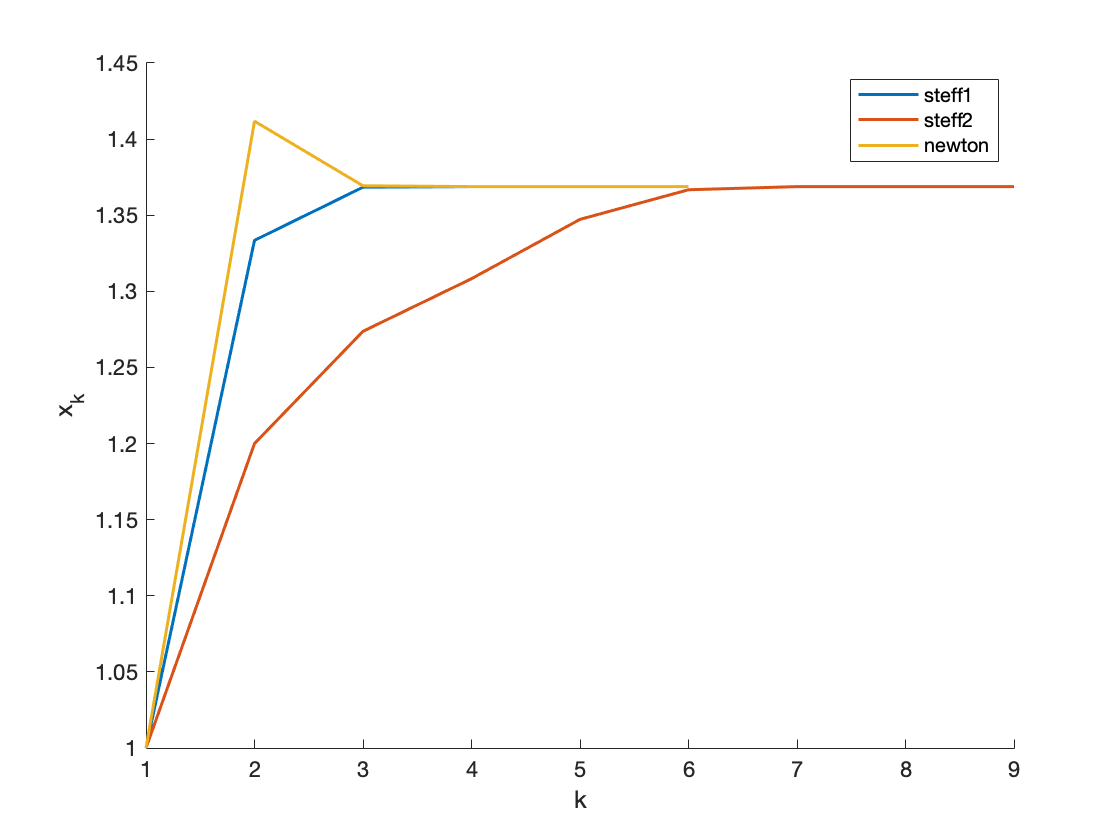
\includegraphics[width = \textwidth]{img/plot3.png} 
		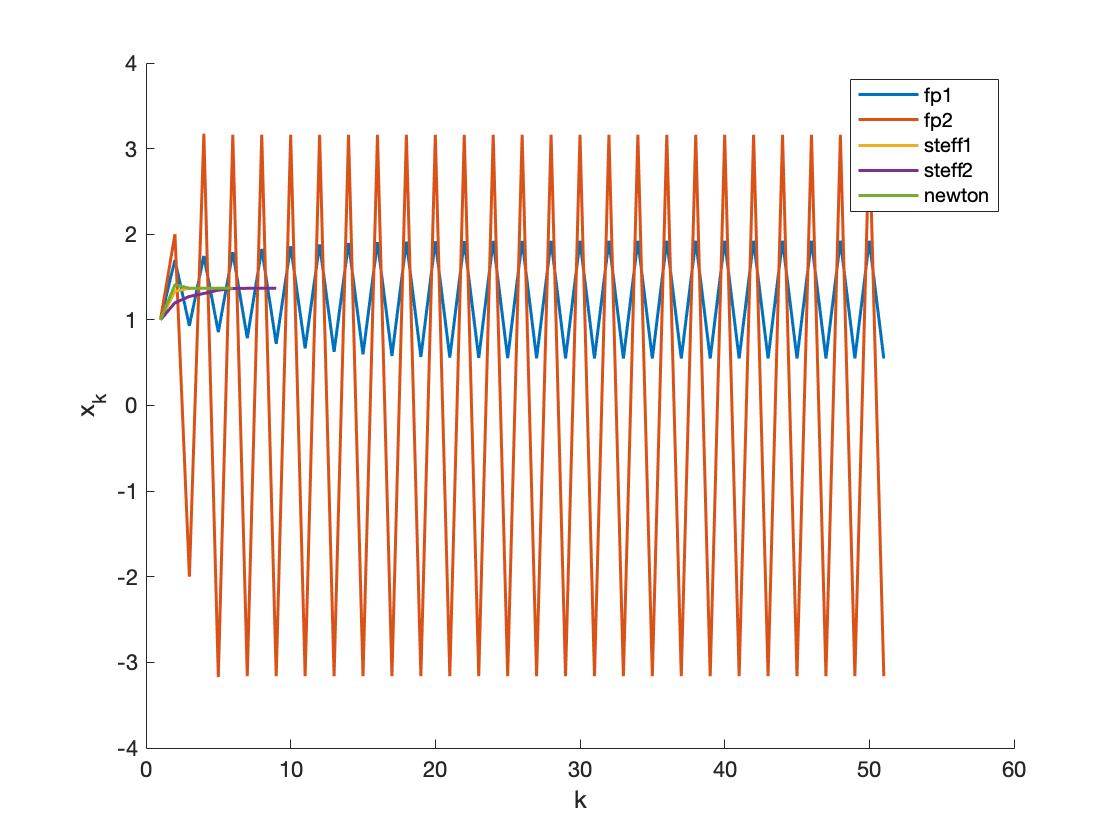
\includegraphics[width = \textwidth]{img/plot5.png} 
		\caption{不同算法的迭代序列}
		\label{plot} 
	\end{figure*}
	
\end{section}

\begin{section}{总结}
	
	本次实验分别采用不动点迭代法、Steffensen 迭代法和 Newton 迭代法求解非线性方程 \ref{equ},并在使用不动点迭代法和 Steffensen 法时分别选取了两种不同的迭代函数 \ref{func1} \ref{func2}。即通过理论分析迭代法的收敛性,又进行编程计算,观察算法产生的迭代序列,得到了与理论相符合的结果。
	
\end{section}

\end{multicols}



%\bibliographystyle{unsrt}
%\bibliography{ref.bib}

%\begin{thebibliography}{99}    %参考文献开始
%	\bibitem{ml}周志华. 机器学习[M]. 清华大学出版社, 2016.   
%\end{thebibliography}	

\end{document}

